\documentclass{article}

% 导入宏包
\usepackage{fancyhdr}
\usepackage{ctex}
\usepackage{listings}
\usepackage{graphicx}
\usepackage[a4paper, body={18cm,22cm}]{geometry}
\usepackage{amsmath,amssymb,amstext,wasysym,enumerate,graphicx}
\usepackage{float,abstract,booktabs,indentfirst,amsmath}
\usepackage{array}
\usepackage{multirow}
\usepackage{url}
\usepackage{diagbox}
\usepackage{enumitem}
\usepackage{xcolor}
\usepackage{makecell}
\usepackage{tikz}
\usetikzlibrary{positioning, arrows.meta}

% 设置段落
\renewcommand\arraystretch{1.4}
\setlength{\parindent}{2em}
\setCJKmonofont{黑体}

% 配置代码显示
\lstset{
	xleftmargin = 3em,
	xrightmargin = 3em,
	aboveskip = 1em,
	backgroundcolor = \color{white},
	basicstyle = \small\ttfamily,
	rulesepcolor = \color{gray},
	breaklines = true,
	numbers = left,
	numberstyle = \small,
	numbersep = -14pt,
	keywordstyle = \color{purple}\bfseries,
	commentstyle = \color{green!60!black}, % 修改注释颜色
	stringstyle = \color{red!60!green!90!blue!90},
	morekeywords = {ASSERT, int64_t, uint32_t},
	moreemph = {ASSERT, NULL},
	emphstyle = \color{red}\bfseries,
	moreemph = [2]{int64\_t, uint32\_t, tid\_t, uint8\_t, int16\_t, uint16\_t, int32\_t, size\_t, bool},
	emphstyle = [2]\color{purple}\bfseries,
	frame = shadowbox,
	showspaces = false,
	columns = fixed
	morecomment = [l][\color{green!60!black}]{+}, % 设置以+开头的代码行为绿色
}

%--------------------页眉--------------------%

\pagestyle{fancy}
\fancyhead[L]{}
\fancyhead[R]{}
\fancyhead[C]{华东师范大学软件工程学院实验报告}
\fancyfoot[C]{-\thepage-}
\renewcommand{\headrulewidth}{1.5pt}

%--------------------标题--------------------%

\begin{document}
	\begin{center}
		{\Large{\textbf{\heiti 华东师范大学软件工程学院实验报告}}}
		\begin{table}[htb]
			\flushleft
			\begin{tabular}{p{0.4\linewidth}p{0.27\linewidth}p{0.28\linewidth}}\\
				\textbf{实验课程}:操作系统实践  & \textbf{年级}:2023级       & \textbf{实验成绩}:  \\
				\textbf{实验名称}:User Programs in Pintos & \textbf{姓名}:顾翌炜         &                 \\
				\textbf{实验编号}:project-2     & \textbf{学号}:10235101527 & \textbf{实验日期}:2024/11/25  \\
				\textbf{指导教师}:陈闻杰     & \textbf{组号}:01            & \textbf{实验时间}:2024/11/25  \\ 
			\end{tabular}
		\end{table}
	\end{center}
	\rule{\textwidth}{2pt}
	
	%--------------------正文--------------------%
	%------------------实验目的------------------%
	
	\section{实验目的}
	
	\begin{enumerate}[noitemsep, label={{\arabic*})}]
		\item 实现参数传递
		\item 实现系统调用
	\end{enumerate}
	
	\section{实验内容以及实验步骤}
	
	为了防止之前的\texttt{Proj-1}对于本次实验的影响,我重新在Docker中导入一个容器,并通过\texttt{git clone https://gitee.com/duerwuyi/pintos.git} 来获取实验相关的材料。
	
	在开始实验之前,cd到\texttt{src/userprog}里面,然后\texttt{make check},得到以下结果:
	
	\begin{figure}[H]
		\centering
		\begin{minipage}[b]{0.45\textwidth}
			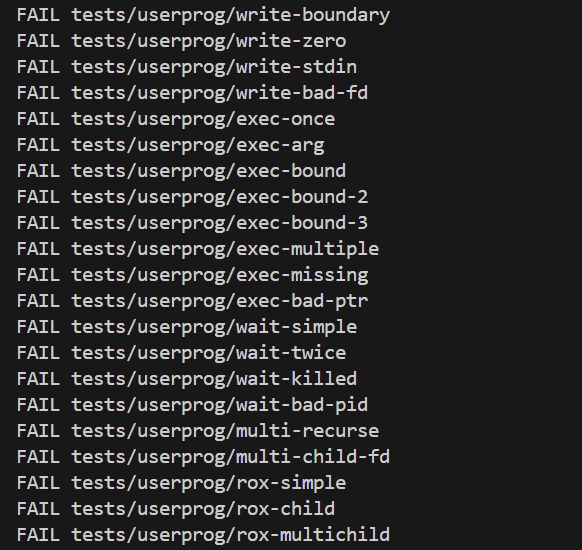
\includegraphics[width=\textwidth]{images/1.before_proj - 1.png}
			\caption{before\_proj - 1}
		\end{minipage}
		\hfill
		\begin{minipage}[b]{0.45\textwidth}
			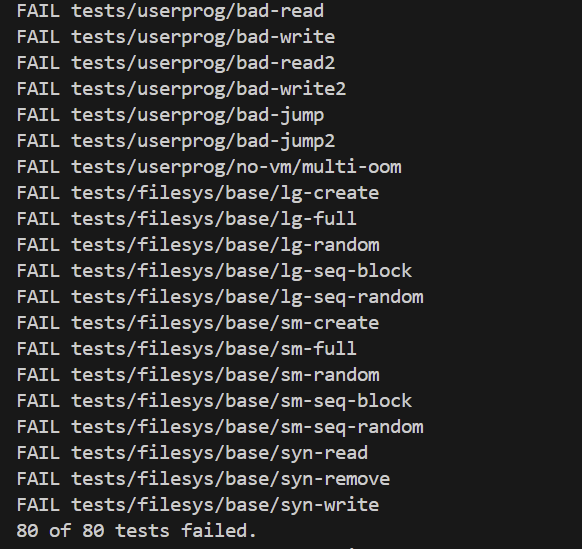
\includegraphics[width=\textwidth]{images/1.before_proj - 2.png}
			\caption{\texttt{before\_proj - 2}}
		\end{minipage}
	\end{figure}
	
	所以本次实验的目的就是完成图中(没有完整截屏)的80个测试点
	
	\subsection{参数传递}
	
	首先,我们需要对线程结构体进行扩展,将添加以下几个关键内容:
	
	\begin{enumerate}
		\item 每个线程的CPU时间估计值等内容
		\item 每个进程的父进程,子进程列表、是否加载成功等内容
		\item 可执行文件以及线程所处的目录等内容
	\end{enumerate}
	
	具体添加在了 \texttt{\#ifdef USERPROG} 之下:
	
	\begin{lstlisting}[xleftmargin = 4em,xrightmargin = 4em, aboveskip = 1em, numbers = left, language = C,title=src/threads/thread.h中的结构体]
    struct thread
    {
    	/* Owned by thread.c. */
    	tid_t tid;                 /* Thread identifier. */
    	enum thread_status status; /* Thread state. */
    	char name[16];  /* Name (for debugging purposes). */
    	uint8_t *stack; /* Saved stack pointer. */
    	int priority;   /* Priority. */
    	
    	int init_priority;
    	struct lock *await_lock;
    	struct list locks_possess_list;
    	
    	struct list_elem allelem; /* List element for all threads list. */
    	
    	/* Shared between thread.c and synch.c. */
    	struct list_elem elem;  /* List element. */
    	int nice;               // 每个线程都有一个整数nice值该值确定该线程与其他线程应该有多“不错”[-20,20]
    	fixed_point recent_cpu; // 线程最近使用的CPU的时间的估计值
    	#ifdef USERPROG
    	/* Owned by userprog/process.c. */
    	uint32_t *pagedir; /* Page directory. */
    	#endif
    	
    	/* Owned by thread.c. */
    	unsigned magic; /* Detects stack overflow. */
    	
    	struct thread *parent;        // 该进程的父进程
    	
    	struct semaphore exec_sema; // 用于父进程等待成功加载子进程的可执行文件时的阻塞
    	bool exec_success;          // 判断加载是否成功
    	
    	struct dir *dir; // 该线程所处的目录位置
    };
	\end{lstlisting}
	
	接下来就是在线程的初始化函数 \texttt{thread\_init()} 中,为线程初始化退出状态、相关数据结构初始化、高级调度程序的相关数据初始化、以及父进程/子进程列表和文件管理列表等进行初始化:
	
	\begin{lstlisting}[xleftmargin = 4em,xrightmargin = 4em, aboveskip = 1em, numbers = left, language = C,title=src/threads/thread.c中初始化函数]
    /* Does basic initialization of T as a blocked thread named
    NAME. */
    /* Does basic initialization of T as a blocked thread named
    NAME. */
    static void
    init_thread(struct thread *t, const char *name, int priority)
    {
    	enum intr_level old_level;
    	
    	ASSERT(t != NULL);
    	ASSERT(PRI_MIN <= priority && priority <= PRI_MAX);
    	ASSERT(name != NULL);
    	
    	memset(t, 0, sizeof *t);
    	t->status = THREAD_BLOCKED;
    	
    	// 为线程初始化退出状态
    	t->exit_code = 0;
    	
    	strlcpy(t->name, name, sizeof t->name);
    	t->stack = (uint8_t *)t + PGSIZE;
    	if (!thread_mlfqs)
    	{
    		t->priority = priority;
    		// 为优先级捐赠相关数据结构进行初始化
    		t->init_priority = priority;
    	}
    	list_init(&t->locks_possess_list);
    	t->await_lock = NULL;
    	// 为高级调度程序初始化相关数据
    	t->recent_cpu = 0;
    	t->nice = 0;
    	
    	t->magic = THREAD_MAGIC;
    	
    	old_level = intr_disable();
    	list_push_back(&all_list, &t->allelem);
    	intr_set_level(old_level);
    	
    	// 为父子进程初始化子进程列表
    	list_init(&t->child_list);
    	// 初始化exec的等待信号量和
    	sema_init(&t->exec_sema, 0);
    	t->exec_success = false;
    	
    	// 初始化文件管理列表
    	list_init(&t->file_list);
    	t->next_fd = 2;
    	// 初始化线程的当前目录参数
    	t->dir = NULL;
    }
	\end{lstlisting}
	
	接下来,我们需要修改\texttt{src/userprog/process.c} 中的\texttt{process\_execute()} 函数,使得其能够将参数传递给新的进程。
	
	\begin{lstlisting}[xleftmargin = 4em,xrightmargin = 4em, aboveskip = 1em, numbers = left, language = C,title=src/userprog/process.c中process\_execute函数]
    /* Starts a new thread running a user program loaded from
    FILENAME.  The new thread may be scheduled (and may even exit)
    before process_execute() returns.  Returns the new process's
    thread id, or TID_ERROR if the thread cannot be created. */
    tid_t process_execute(const char *file_name)
    {
    	char *fn_for_process_name, *fn_for_start_process_arguments;
    	tid_t tid;
    	
    	// 为FILE_NAME生成两份拷贝,其中一份用于线程名,另一份用于start_process的参数
    	// 目的主要是为了避免发生访存冲突
    	fn_for_process_name = palloc_get_page(0);
    	fn_for_start_process_arguments = palloc_get_page(0);
    	if (fn_for_process_name == NULL || fn_for_start_process_arguments == NULL)
    	return TID_ERROR;
    	strlcpy(fn_for_process_name, file_name, PGSIZE);
    	strlcpy(fn_for_start_process_arguments, file_name, PGSIZE);
    	
    	// 通过Pintos文档提示的strtok_r函数来分割字符串
    	char *save_ptr;
    	char *process_name = strtok_r(fn_for_process_name, " ", &save_ptr);
    	// 将分割后的字符串用于线程名称的赋值,将另一份拷贝用于start_process进行处理
    	tid = thread_create(process_name, PRI_DEFAULT, start_process, fn_for_start_process_arguments);
    	if (tid == TID_ERROR)
    	{
    		palloc_free_page(fn_for_process_name);
    		palloc_free_page(fn_for_start_process_arguments);
    	}
    	// 将当前线程阻塞
    	sema_down(&thread_current()->exec_sema);
    	// 如果子进程运行失败了那么就返回-1
    	if (!thread_current()->exec_success)
    	{
    		return -1;
    	}
    	// 重置执行参数以便下一次调用
    	thread_current()->exec_success = false;
    	palloc_free_page(fn_for_process_name);
    	return tid;
    }
	\end{lstlisting}
	
	来解释一下这个函数修改的思路:
	
	在这个函数中,首先启动一个新线程来运行指定文件名的用户程序。它首先创建文件名的两个副本,以避免在线程创建和执行过程中对原始字符串的修改。然后,函数使用 \texttt{strtok\_r} 分割文件名以获取程序名,并创建一个新线程。如果线程创建失败,会释放内存并返回错误。创建线程后,当前线程会等待新线程的执行结果。如果新线程执行失败,函数返回 \texttt{-1};否则,释放资源并返回新线程的ID。这个设计确保了父线程能够及时了解子线程的执行状态,并有效管理资源。\\
	
	接下来,我们需要修改\texttt{src/userprog/process.c} 中的\texttt{start\_process()} 函数,使得其能够将参数压入栈中。
	
	下表显示了在用户程序开始之前堆栈和相关寄存器的状态,假设 \texttt{PHYS\_BASE} 为 \texttt{0xc0000000}。
	
	\clearpage
	
	\begin{table}[htb]
		\centering
		\begin{tabular}{cccc}
			\textbf{Address} & \textbf{Name} & \textbf{Data} & \textbf{Type} \\
			0xbfffffc & argv[3][...] & "bar\textbackslash{}0" & char[4] \\
			0xbfffff8 & argv[2][...] & "foo\textbackslash{}0" & char[4] \\
			0xbfffff5 & argv[1][...] & "-1\textbackslash{}0" & char[3] \\
			0xbfffffd & argv[0][...] & "/bin/ls\textbackslash{}0" & char[8] \\
			0xbffffece & word-align & 0 & uint8\_t \\
			0xbfffff8 & argv[4] & 0 & char * \\
			0xbfffffe4 & argv[3] & 0xbfffffc & char * \\
			0xbfffffe0 & argv[2] & 0xbfffff8 & char * \\
			0xbfffffdc & argv[1] & 0xbfffff5 & char * \\
			0xbfffffd8 & argv[0] & 0xbfffffd & char * \\
			0xbfffffd4 & argv & 0xbfffffd8 & char ** \\
			0xbfffffd0 & argc & 4 & int \\
			0xbfffffc & return address & 0 & void (*)() \\
		\end{tabular}
		\caption{表1: 压入参数的顺序和结构} % 为表格添加标题
	\end{table}
	
	\setlength{\parindent}{2em}
	
	在这个例子中,堆栈指针将被初始化为 \texttt{0xbfffffcc}。
	
	以这个为例,接下来需要完善的是在 \texttt{start\_process()} 函数,首先来看一下原本的 \texttt{start\_process()} 函数
	
	\begin{lstlisting}[xleftmargin = 4em,xrightmargin = 4em, aboveskip = 1em, numbers = left, language = C,title=原本的src/userprog/process.c - start\_process]
    /* A thread function that loads a user process and starts it
    running. */
    static void start_process(void *file_name_)
    {
    	char *file_name = file_name_;
    	struct intr_frame if_;
    	bool success;
    	
    	/* Initialize interrupt frame. */
    	memset(&if_, 0, sizeof if_);
    	if_.gs = if_.fs = if_.es = if_.ds = if_.ss = SEL_UDSEG;
    	if_.cs = SEL_UCSEG;
    	if_.eflags = FLAG_IF | FLAG_MBS;
    	
    	/* Load executable. */
    	char *save_ptr;
    	char *cmd = strtok_r(file_name, " ", &save_ptr);
    	success = load(cmd, &if_.eip, &if_.esp);
    	
    	if (success)
    	{
    		if_.esp = arg_pass((esp_t)if_.esp, cmd, save_ptr);
    		process_load_success(cmd);
    	}
    	
    	/* Free file_name whether successed or failed. */
    	palloc_free_page(file_name);
    	
    	if (!success)
    	{
    		process_load_fail();
    		NOT_REACHED();
    	}
    	
    	/* Start the user process by simulating a return from an
    	interrupt, implemented by intr_exit (in
    	threads/intr-stubs.S).  Because intr_exit takes all of its
    	arguments on the stack in the form of a `struct intr_frame',
    	we just point the stack pointer (%esp) to our stack frame
    	and jump to it. */
    	asm volatile(
    	"movl %0, %%esp; \
    	jmp intr_exit"
    	:
    	: "g"(&if_)
    	: "memory");
    	NOT_REACHED();
    }
	\end{lstlisting}
	
	可以看出:`start\_process` 函数作为线程函数,负责加载用户进程并启动其执行。它初始化中断帧,设置段寄存器和标志,然后调用 `load` 函数加载程序。如果加载失败,函数会释放资源并退出。成功加载后,通过模拟中断返回,将控制权交给用户程序的入口点,从而启动进程。\\
	
	我的新的函数实现思路是:`start\_process` 函数负责加载并启动一个用户程序。它首先为程序名和参数分配内存并复制文件名,然后初始化中断帧以准备线程状态。函数尝试加载可执行文件,如果失败则设置错误状态并退出。成功后,它设置成功标志并继续解析命令行参数,将它们压入栈中以供程序使用。
	
	接着,函数确保正在运行的可执行文件不可被修改,并通过设置文件的写入权限来实现。之后,它为线程设置目录(如果尚未设置),并清理分配的内存。最后,通过模拟中断返回,函数启动用户程序,使用 `intr\_exit` 来转移控制权,从而开始执行用户代码。这个过程确保了用户程序在受控环境中启动,同时保护了系统资源。
	
	
	\begin{lstlisting}[xleftmargin = 4em,xrightmargin = 4em, aboveskip = 1em, numbers = left, language = C,title=修改后的src/userprog/process.c - start\_process]
    /* A thread function that loads a user process and starts it
    running. */
    static void
    start_process(void *file_name_)
    {
    	char *fn_for_process_name = file_name_, *fn_for_start_process_arguments;
    	fn_for_start_process_arguments = palloc_get_page(0);
    	strlcpy(fn_for_start_process_arguments, fn_for_process_name, PGSIZE);
    	struct intr_frame if_;
    	bool success;
    	
    	char *token, *save_ptr;
    	char *process_name = strtok_r(fn_for_process_name, " ", &save_ptr);
    	
    	/* Initialize interrupt frame and load executable. */
    	memset(&if_, 0, sizeof if_);
    	if_.gs = if_.fs = if_.es = if_.ds = if_.ss = SEL_UDSEG;
    	if_.cs = SEL_UCSEG;
    	if_.eflags = FLAG_IF | FLAG_MBS;
    	
    	lock_acquire(&filesys_lock);
    	success = load(process_name, &if_.eip, &if_.esp);
    	lock_release(&filesys_lock);
    	
    	if (!success)
    	{
    		// 如果执行失败就将子进程的状态设置为结束状态同时设置状态码为-1并唤醒父进程
    		thread_current()->as_child->is_alive = false;
    		thread_current()->exit_code = -1;
    		sema_up(&thread_current()->parent->exec_sema);
    		palloc_free_page(fn_for_process_name);
    		palloc_free_page(fn_for_start_process_arguments);
    		thread_exit();
    	} // 如果执行成功就将父进程的执行成功标识符置为true并唤醒父进程
    	thread_current()->parent->exec_success = 1;
    	sema_up(&thread_current()->parent->exec_sema);
    	int argc = 0;
    	void *argv[128];
    	// 第一步:将栈指针指向用户虚拟地址空间的开头
    	if_.esp = PHYS_BASE;
    	// 第二步:解析参数,将它们放置在栈顶并记录他们的地址,此处单词的顺序无关紧要
    	for (token = strtok_r(fn_for_start_process_arguments, " ", &save_ptr); token != NULL; token = strtok_r(NULL, " ", &save_ptr))
    	{
    		size_t arg_len = strlen(token) + 1; // strlen不算\0因此需要+1
    		if_.esp -= arg_len;
    		memcpy(if_.esp, token, arg_len);
    		argv[argc++] = if_.esp;
    	}
    	// 第三步:首先将指针向下舍入到4的倍数,然后推送每个字符串的地址
    	uintptr_t temp = (uintptr_t)if_.esp; // 指针不能直接进行取模运行
    	if (temp % 4 != 0)
    	{
    		temp -= temp % 4;
    	}
    	if_.esp = (void *)temp; // 这一步注意不要漏了
    	// 第四步:加上堆栈上的空指针哨兵,按从右到左的顺序。
    	size_t ptr_size = sizeof(void *);
    	if_.esp -= ptr_size;
    	memset(if_.esp, 0, ptr_size);
    	for (int i = argc - 1; i >= 0; i--)
    	{
    		if_.esp -= ptr_size;
    		memcpy(if_.esp, &argv[i], ptr_size);
    		// printf("%s\n",argv[i]);
    	}
    	// 第五步:将argv的地址即argv[0]压入栈中,使得程序能够在后续访问到上述参数
    	if_.esp -= ptr_size;
    	*(uintptr_t *)if_.esp = ((uintptr_t)if_.esp + ptr_size);
    	// 将argc压入栈中,使得程序能够在后续访问到参数的个数
    	if_.esp -= ptr_size;
    	*(int *)if_.esp = argc;
    	// 第六步:压入一个返回地址
    	if_.esp -= ptr_size;
    	memset(if_.esp, 0, ptr_size);
    	// 文档提示我们使用`hex_dump()`函数来打印内存状况以检验实现的正确性
    	// printf("STACK SET. ESP: %p\n", if_.esp);
    	// hex_dump((uintptr_t)if_.esp, if_.esp, 100, true); // 打印的byte数不用特别准确,随便填大一些
    	
    	// 一个进程自己正在运行的可执行文件不应该能够被修改于是将自己的可执行文件打开并存入该指针来拒绝写入
    	lock_acquire(&filesys_lock);
    	struct file *f = filesys_open(process_name);
    	file_deny_write(f);
    	lock_release(&filesys_lock);
    	thread_current()->exec_file = f;
    	
    	palloc_free_page(fn_for_process_name);
    	palloc_free_page(fn_for_start_process_arguments);
    	// 如果当前线程没有设置目录那么就将根目录设置为其目录
    	if (!thread_current()->dir)
    	thread_current()->dir = dir_open_root();
    	/* Start the user process by simulating a return from an
    	interrupt, implemented by intr_exit (in
    	threads/intr-stubs.S).  Because intr_exit takes all of its
    	arguments on the stack in the form of a `struct intr_frame',
    	we just point the stack pointer (%esp) to our stack frame
    	and jump to it. */
    	asm volatile("movl %0, %%esp; jmp intr_exit"
    	:
    	: "g"(&if_)
    	: "memory");
    	NOT_REACHED();
    }
	\end{lstlisting}
	
	到这里,参数传递的实现就完成了。我们可以尝试运行一个测试用例:
	
	
	\begin{lstlisting}[xleftmargin = 4em,xrightmargin = 4em, aboveskip = 1em, numbers = left, language = C,title=测试用例]
    $ pintos -v -k -T 60 --qemu --filesys-size=2 -p build/tests/userprog/args-none -a args-none -- -q -f run args-none
    SeaBIOS (version 1.15.0-1)
    Booting from Hard Disk...
    PPiiLLoo hddaa1
    1
    LLooaaddiinngg...
    Kernel command line: -q -f extract run 'args-single onearg'
    Pintos booting with 3,968 kB RAM...
    367 pages available in kernel pool.
    367 pages available in user pool.
    Calibrating timer... 556,236,800 loops/s.
    ide0: unexpected interrupt
    hda: 5,040 sectors (2 MB), model "QM00001", serial "QEMU HARDDISK"
    hda1: 195 sectors (97 kB), Pintos OS kernel (20)
    hda2: 4,096 sectors (2 MB), Pintos file system (21)
    hda3: 117 sectors (58 kB), Pintos scratch (22)
    ide1: unexpected interrupt
    filesys: using hda2
    scratch: using hda3
    Formatting file system...done.
    Boot complete.
    Extracting ustar archive from scratch device into file system...
    Putting 'args-single' into the file system...
    Erasing ustar archive...
    Executing 'args-single onearg':
    system call!
    Execution of 'args-single onearg' complete.
    Timer: 71 ticks
    Thread: 8 idle ticks, 63 kernel ticks, 0 user ticks
    hda2 (filesys): 63 reads, 238 writes
    hda3 (scratch): 116 reads, 2 writes
    Console: 930 characters output
    Keyboard: 0 keys pressed
    Exception: 0 page faults
    Powering off...
	\end{lstlisting}
	
	在这个用例中输出了system call!,这是由于我们暂时还没有实现相关的系统调用。
	
	所以接下来继续完成系统调用的任务。
	
	\subsection{系统调用}
	
	首先,我们在 \texttt{src/userprog/syscall.c} 中声明相关函数
	
	\begin{lstlisting}[xleftmargin = 4em,xrightmargin = 4em, aboveskip = 1em, numbers = left, language = C,title=\texttt{src/userprog/syscall.c} 中声明相关函数]
    static void syscall_handler(struct intr_frame *);
    static void syscall_halt(struct intr_frame *) NO_RETURN;
    static void syscall_exit(struct intr_frame *) NO_RETURN;
    static void syscall_exec(struct intr_frame *);
    static void syscall_wait(struct intr_frame *);
    
    static void syscall_create(struct intr_frame *);
    static void syscall_remove(struct intr_frame *);
    static void syscall_open(struct intr_frame *);
    static void syscall_filesize(struct intr_frame *);
    static void syscall_read(struct intr_frame *);
    static void syscall_write(struct intr_frame *);
    static void syscall_seek(struct intr_frame *);
    static void syscall_tell(struct intr_frame *);
    static void syscall_close(struct intr_frame *);
	\end{lstlisting}
	
	然后在 \texttt{syscall\_init()} 函数中初始化相关系数,并且调用 \texttt{syscall\_handler} 来调用需要的函数:
	
	\begin{lstlisting}[xleftmargin = 4em,xrightmargin = 4em, aboveskip = 1em, numbers = left, language = C,title=初始化函数]
    void syscall_init(void)
    {
    	intr_register_int(0x30, 3, INTR_ON, syscall_handler, "syscall");
    }
	\end{lstlisting}
	
	在执行系统调用过程中,为了访问用户空间的内存,我们必须确保内存访问的合法性。为此,我们开发了两个关键函数:\texttt{get\_user()}和\texttt{check\_read\_user\_ptr()}。这些函数的目的是验证用户空间内存的有效性。如果检测到内存访问违规,我们通过调用\texttt{terminate\_process}函数来终止当前进程,并返回错误代码\texttt{-1}。
	
	\begin{lstlisting}[xleftmargin = 4em,xrightmargin = 4em, aboveskip = 1em, numbers = left, language = C,title=src/userprog/syscall.c - \texttt{get\_user()}]
    // 从用户虚拟地址空间中读取一个字节的信息,如果成功那么就返回该信息否则返回-1
    static int
    get_user(const uint8_t *uaddr)
    {
    	int result;
    	asm("movl $1f, %0; movzbl %1, %0; 1:"
    	    : "=&a"(result)
    	    : "m"(*uaddr));
    	return result;
    }
	\end{lstlisting}
	
	\begin{lstlisting}[xleftmargin = 4em,xrightmargin = 4em, aboveskip = 1em, numbers = left, language = C,title=src/syscall.c - \texttt{check\_read\_user\_ptr()}]
    // 检查一个用户提供的指针是否能够合法读取数据,如果合法就返回该指针否则就调用terminate_process
    static void *
    check_read_user_ptr(const void *ptr, size_t size)
    {
    	if (!is_user_vaddr(ptr))
    	{
    		terminate_process();
    	}
    	for (size_t i = 0; i < size; i++)
    	{ // check if every byte is safe to read
    		if (get_user(ptr + i) == -1)
    		{
    			terminate_process();
    		}
    	}
    	return (void *)ptr; // remove const
    }
	\end{lstlisting}
	
	\begin{lstlisting}[xleftmargin = 4em,xrightmargin = 4em, aboveskip = 1em, numbers = left, language = C,title=src/userprog/syscall.c - \texttt{terminate\_process()}]
    // 终止一个进程
    static void
    terminate_process(void)
    {
    	thread_current()->exit_code = -1;
    	thread_exit();
    	NOT_REACHED();
    }
	\end{lstlisting}
	
	在这里,为了存储线程的退出状态,所以我们需要在线程结构体中添加int exit\_status。
	
	\begin{lstlisting}[xleftmargin = 4em,xrightmargin = 4em, aboveskip = 1em, numbers = left, language = C,title=src/threads/thread.h中的结构体]
    struct thread
    {
    	/* Owned by thread.c. */
    	tid_t tid;                 /* Thread identifier. */
    	enum thread_status status; /* Thread state. */
    	int exit_code;
    	char name[16];  /* Name (for debugging purposes). */
    	uint8_t *stack; /* Saved stack pointer. */
    	int priority;   /* Priority. */
    	
    	int init_priority;
    	struct lock *await_lock;
    	struct list locks_possess_list;
    	
    	struct list_elem allelem; /* List element for all threads list. */
    	
    	/* Shared between thread.c and synch.c. */
    	struct list_elem elem;  /* List element. */
    	int nice;               // 每个线程都有一个整数nice值该值确定该线程与其他线程应该有多“不错”[-20,20]
    	fixed_point recent_cpu; // 线程最近使用的CPU的时间的估计值
    	#ifdef USERPROG
    	/* Owned by userprog/process.c. */
    	uint32_t *pagedir; /* Page directory. */
    	#endif
    	
    	/* Owned by thread.c. */
    	unsigned magic; /* Detects stack overflow. */
    	
    	struct thread *parent;        // 该进程的父进程
    	
    	struct semaphore exec_sema; // 用于父进程等待成功加载子进程的可执行文件时的阻塞
    	bool exec_success;          // 判断加载是否成功
    	
    	struct dir *dir; // 该线程所处的目录位置
    };
	\end{lstlisting}
	
	接下来,修改src/userprog/exception.c中的page\_fault() 函数,使得其能够处理用户空间的内存错误。
	
	\begin{lstlisting}[xleftmargin = 4em,xrightmargin = 4em, aboveskip = 1em, numbers = left, language = C,title=src/userprog/syscall.c - \texttt{page\_fault()}]
    /* Page fault handler.  This is a skeleton that must be filled in
    to implement virtual memory.  Some solutions to project 2 may
    also require modifying this code.
    
    At entry, the address that faulted is in CR2 (Control Register
    2) and information about the fault, formatted as described in
    the PF_* macros in exception.h, is in F's error_code member.  The
    example code here shows how to parse that information.  You
    can find more information about both of these in the
    description of "Interrupt 14--Page Fault Exception (#PF)" in
    [IA32-v3a] section 5.15 "Exception and Interrupt Reference". */
    static void
    page_fault (struct intr_frame *f) 
    {
    	bool not_present;  /* True: not-present page, false: writing r/o page. */
    	bool write;        /* True: access was write, false: access was read. */
    	bool user;         /* True: access by user, false: access by kernel. */
    	void *fault_addr;  /* Fault address. */
    	
    	/* Obtain faulting address, the virtual address that was
    	accessed to cause the fault.  It may point to code or to
    	data.  It is not necessarily the address of the instruction
    	that caused the fault (that's f->eip).
    	See [IA32-v2a] "MOV--Move to/from Control Registers" and
    	[IA32-v3a] 5.15 "Interrupt 14--Page Fault Exception
    	(#PF)". */
    	asm ("movl %%cr2, %0" : "=r" (fault_addr));
    	
    	/* Turn interrupts back on (they were only off so that we could
    	be assured of reading CR2 before it changed). */
    	intr_enable ();
    	
    	/* Count page faults. */
    	page_fault_cnt++;
    	
    	/* Determine cause. */
    	not_present = (f->error_code & PF_P) == 0;
    	write = (f->error_code & PF_W) != 0;
    	user = (f->error_code & PF_U) != 0;
    	
    	//对于内核态的代码如果没有明显的逻辑错误是不会进入页面错误中断的
    	//于是可以简单的认为如果在内核态发生了页面错误那就是syscall
    	if(!user){
    		//强转为返回值为void但是没有参数的函数指针
    		f->eip=(void(*)(void))f->eax;
    		f->eax=-1;
    		return;
    	}
    	/* To implement virtual memory, delete the rest of the function
    	body, and replace it with code that brings in the page to
    	which fault_addr refers. */
    	printf ("Page fault at %p: %s error %s page in %s context.\n",
    	fault_addr,
    	not_present ? "not present" : "rights violation",
    	write ? "writing" : "reading",
    	user ? "user" : "kernel");
    	kill (f);
    }
	\end{lstlisting}
	
	接下来,我们来实现 \texttt{syscall\_handler()} 函数,来处理系统调用
	
	\begin{lstlisting}[xleftmargin = 4em,xrightmargin = 4em, aboveskip = 1em, numbers = left, language = C,title=src/userprog/syscall.c - \texttt{page\_fault()}]
    // 在用户的中断处理程序中解析系统调用的符号
    // 根据类型分发给各个具体处理函数逐个实现
    static void
    syscall_handler(struct intr_frame *f UNUSED)
    {
    	int syscall_type = *(int *)check_read_user_ptr(f->esp, sizeof(int));
    	switch (syscall_type)
    	{
    		case SYS_HALT:
    		syscall_halt(f);
    		break;
    		case SYS_EXIT:
    		syscall_exit(f);
    		break;
    		case SYS_EXEC:
    		syscall_exec(f);
    		break;
    		case SYS_WAIT:
    		syscall_wait(f);
    		break;
    		case SYS_CREATE:
    		syscall_create(f);
    		break;
    		case SYS_REMOVE:
    		syscall_remove(f);
    		break;
    		case SYS_OPEN:
    		syscall_open(f);
    		break;
    		case SYS_FILESIZE:
    		syscall_filesize(f);
    		break;
    		case SYS_READ:
    		syscall_read(f);
    		break;
    		case SYS_WRITE:
    		syscall_write(f);
    		break;
    		case SYS_SEEK:
    		syscall_seek(f);
    		break;
    		case SYS_TELL:
    		syscall_tell(f);
    		break;
    		case SYS_CLOSE:
    		syscall_close(f);
    		break;
    		case SYS_CHDIR:
    		syscall_chdir(f);
    		break;
    		case SYS_MKDIR:
    		syscall_mkdir(f);
    		break;
    		case SYS_READDIR:
    		syscall_readdir(f);
    		break;
    		case SYS_ISDIR:
    		syscall_isdir(f);
    		break;
    		case SYS_INUMBER:
    		syscall_inumber(f);
    		break;
    		default:
    		NOT_REACHED();
    		break;
    	}
    }
	\end{lstlisting}
	
	接下来就是实现相关系统调用函数的实现了:
	
	\subsubsection{syscall\_halt()}
	
	\textbf{syscall\_halt()}函数用于关闭系统:
	
	\begin{lstlisting}[xleftmargin = 4em,xrightmargin = 4em, aboveskip = 1em, numbers = left, language = C,title=src/userprog/syscall.c - \texttt{syscall\_halt()}]
    static void
    syscall_halt(struct intr_frame *f UNUSED)
    {
    	shutdown_power_off();
    }
	\end{lstlisting}
	
	\subsubsection{syscall\_exit()}
	
	\textbf{syscall\_exit()}函数用于退出进程:
	
	\begin{lstlisting}[xleftmargin = 4em,xrightmargin = 4em, aboveskip = 1em, numbers = left, language = C,title=src/userprog/syscall.c - \texttt{syscall\_exit()}]
    static void
    syscall_exit(struct intr_frame *f)
    {
    	// exit_code在系统调用之后被解析为参数
    	int exit_code = *(int *)check_read_user_ptr(f->esp + ptr_size, sizeof(int));
    	thread_current()->exit_code = exit_code;
    	thread_exit();
    }
	\end{lstlisting}
	
	\subsubsection{syscall\_exec()}
	
	\textbf{syscall\_exec()}函数用于执行程序:
	
	\begin{lstlisting}[xleftmargin = 4em,xrightmargin = 4em, aboveskip = 1em, numbers = left, language = C,title=src/userprog/syscall.c - \texttt{syscall\_exec()}]
    // 运行其名称在 cmd_line 中给出的可执行文件,并传递任何给定的参数,返回新进程的进程ID(pid)
    static void
    syscall_exec(struct intr_frame *f)
    {
    	char *cmd_line = *(char **)check_read_user_ptr(f->esp + ptr_size, ptr_size);
    	check_read_user_str(cmd_line);
    	f->eax = process_execute(cmd_line);
    }
	\end{lstlisting}
	
	\subsubsection{syscall\_wait()}
	
	\textbf{syscall\_wait()}函数用于等待子进程执行完毕:
	
	\begin{lstlisting}[xleftmargin = 4em,xrightmargin = 4em, aboveskip = 1em, numbers = left, language = C,title=src/userprog/syscall.c - \texttt{syscall\_wait()}]
    // 获取pid参数并调用process_wait
    static void
    syscall_wait(struct intr_frame *f)
    {
    	int pid = *(int *)check_read_user_ptr(f->esp + ptr_size, sizeof(int));
    	f->eax = process_wait(pid);
    }
	\end{lstlisting}
	
	在这里,我们需要修改src/userprog/process.c 中的process\_wait() 函数,使得其能够等待子进程执行完毕。
	
	首先,我们需要修改线程结构体,添加struct list child\_list;,用于存放子进程的线程结构体,以及定义子线程结构体struct child\_entry *as\_child;,用于存放子进程的信息。
	
	\begin{lstlisting}[xleftmargin = 4em,xrightmargin = 4em, aboveskip = 1em, numbers = left, language = C,title=src/threads/thread.h - thread结构体]
    struct thread
    {
    	/* Owned by thread.c. */
    	tid_t tid;                 /* Thread identifier. */
    	enum thread_status status; /* Thread state. */
    	int exit_code;
    	char name[16];  /* Name (for debugging purposes). */
    	uint8_t *stack; /* Saved stack pointer. */
    	int priority;   /* Priority. */
    	
    	int init_priority;
    	struct lock *await_lock;
    	struct list locks_possess_list;
    	
    	struct list_elem allelem; /* List element for all threads list. */
    	
    	/* Shared between thread.c and synch.c. */
    	struct list_elem elem;  /* List element. */
    	int nice;               // 每个线程都有一个整数nice值该值确定该线程与其他线程应该有多“不错”[-20,20]
    	fixed_point recent_cpu; // 线程最近使用的CPU的时间的估计值
    	#ifdef USERPROG
    	/* Owned by userprog/process.c. */
    	uint32_t *pagedir; /* Page directory. */
    	#endif
    	
    	/* Owned by thread.c. */
    	unsigned magic; /* Detects stack overflow. */
    	
    	struct thread *parent;        // 该进程的父进程
    	struct list child_list;       // 该进程的子进程列表,每一个元素为child_entry类型的
    	struct child_entry *as_child; // 该进程本身作为子进程时维护的结构
    	
    	struct semaphore exec_sema; // 用于父进程等待成功加载子进程的可执行文件时的阻塞
    	bool exec_success;          // 判断加载是否成功
    	
    	struct dir *dir; // 该线程所处的目录位置
    };
	\end{lstlisting}
	
	再接下来,需要在 \texttt{create\_thread()} 函数和 \texttt{init\_thread()} 函数中初始化这些变量:
	
	\begin{lstlisting}[xleftmargin = 4em,xrightmargin = 4em, aboveskip = 1em, numbers = left, language = C,title=src/threads/thread.c - create\_thread()]
    tid_t thread_create(const char *name, int priority,
    thread_func *function, void *aux)
    {
    	struct thread *t;
    	struct kernel_thread_frame *kf;
    	struct switch_entry_frame *ef;
    	struct switch_threads_frame *sf;
    	tid_t tid;
    	
    	ASSERT(function != NULL);
    	
    	/* Allocate thread. */
    	t = palloc_get_page(PAL_ZERO);
    	if (t == NULL)
    	return TID_ERROR;
    	
    	/* Initialize thread. */
    	init_thread(t, name, priority);
    	tid = t->tid = allocate_tid();
    	// 为父子进程相关的结构和其参数初始化
    	t->as_child = malloc(sizeof(struct child_entry));
    	t->as_child->tid = tid;
    	t->as_child->t = t;
    	t->as_child->is_alive = true;
    	t->as_child->exit_code = 0;
    	t->as_child->is_waiting_on = false;
    	sema_init(&t->as_child->wait_sema, 0);
    	// 将该进程与创建该进程的父进程相链接
    	t->parent = thread_current();
    	list_push_back(&t->parent->child_list, &t->as_child->elem);
    	/* Stack frame for kernel_thread(). */
    	kf = alloc_frame(t, sizeof *kf);
    	kf->eip = NULL;
    	kf->function = function;
    	kf->aux = aux;
    	
    	/* Stack frame for switch_entry(). */
    	ef = alloc_frame(t, sizeof *ef);
    	ef->eip = (void (*)(void))kernel_thread;
    	
    	/* Stack frame for switch_threads(). */
    	sf = alloc_frame(t, sizeof *sf);
    	sf->eip = switch_entry;
    	sf->ebp = 0;
    	// 为当前线程设置目录
    	if (thread_current()->dir)
    	t->dir = dir_reopen(thread_current()->dir);
    	else
    	t->dir = NULL;
    	
    	/* Add to run queue. */
    	thread_unblock(t);
    	// 对于开中断来说只需要在新建线程的优先级大于当前线程时进行让步重新调度即可
    	if (priority > thread_current()->priority)
    	{
    		thread_yield();
    	}
    	
    	return tid;
    }
	\end{lstlisting}
	
	\begin{lstlisting}[xleftmargin = 4em,xrightmargin = 4em, aboveskip = 1em, numbers = left, language = C,title=src/threads/thread.c - init\_thread()]
    /* Does basic initialization of T as a blocked thread named
    NAME. */
    static void
    init_thread(struct thread *t, const char *name, int priority)
    {
    	enum intr_level old_level;
    	
    	ASSERT(t != NULL);
    	ASSERT(PRI_MIN <= priority && priority <= PRI_MAX);
    	ASSERT(name != NULL);
    	
    	memset(t, 0, sizeof *t);
    	t->status = THREAD_BLOCKED;
    	
    	// 为线程初始化退出状态
    	t->exit_code = 0;
    	
    	strlcpy(t->name, name, sizeof t->name);
    	t->stack = (uint8_t *)t + PGSIZE;
    	if (!thread_mlfqs)
    	{
    		t->priority = priority;
    		// 为优先级捐赠相关数据结构进行初始化
    		t->init_priority = priority;
    	}
    	list_init(&t->locks_possess_list);
    	t->await_lock = NULL;
    	// 为高级调度程序初始化相关数据
    	t->recent_cpu = 0;
    	t->nice = 0;
    	
    	t->magic = THREAD_MAGIC;
    	
    	old_level = intr_disable();
    	list_push_back(&all_list, &t->allelem);
    	intr_set_level(old_level);
    	
    	// 为父子进程初始化子进程列表
    	list_init(&t->child_list);
    	// 初始化exec的等待信号量和
    	sema_init(&t->exec_sema, 0);
    	t->exec_success = false;
    }
	\end{lstlisting}
	
	还需要修改的是 \texttt{process\_wait()} 函数:
	
	\begin{lstlisting}[xleftmargin = 4em,xrightmargin = 4em, aboveskip = 1em, numbers = left, language = C,title=src/userprog/process.c - process\_wait]
    int process_wait(tid_t child_tid)
    {
        struct thread *current_thread = thread_current(); //
        struct list_elem *elem_;
        // 遍历当前进程的所有子进程
        for (elem_ = list_begin(&current_thread->child_list); elem_ != list_end(&current_thread->child_list); elem_ = list_next(elem_))
        {
            struct child_entry *entry = list_entry(elem_, struct child_entry, elem);
            // 如果存在进程所需要等待的子进程tid
            if (entry->tid == child_tid)
            {
            	// 如果该子进程并没有被父进程所等待同时子进程并没有结束那么就使用信号量卡住自身来等待子进程运行结束
            	if (!entry->is_waiting_on && entry->is_alive)
            	{
                    entry->is_waiting_on = true;
                    sema_down(&entry->wait_sema);
                    return entry->exit_code;
            	}
            	else if (entry->is_waiting_on)
            	{ // 如果已经在等待该子进程了那么就返回-1
            	    return -1;
            	}
            	else
            	{ // 如果子进程已经结束那么就返回exit_code
            	    return entry->exit_code;
            	}
            }
        }
        return -1;
    }
	\end{lstlisting}
	
	在本函数的实现中,我们首要任务是审查当前线程的所有子线程。通过识别特定的子线程,我们进一步评估其执行状态。若子线程已完成执行,我们将获取并报告其终止状态;若未完成,函数将返回 \texttt{-1} 。
	
	此外,我们对\texttt{thread\_exit()}函数进行了必要的调整。这些调整确保了在子线程结束时,父进程能够得到唤醒。
	
	\subsubsection{syscall\_write}
	
	\texttt{write()} 函数负责将数据写入文件。
	
	为实现文件操作,我们在线程结构体中增加了 \texttt{struct file *exec\_file;} 以管理由线程创建的可执行文件,并引入 \texttt{struct list file\_list} 来记录该线程的可执行文件列表,每一个元素为file\_entry。同时,定义了 \texttt{next\_fd} 来存储下一个被分配的文件描述符。
	
	\begin{lstlisting}[xleftmargin = 4em,xrightmargin = 4em, aboveskip = 1em, numbers = left, language = C,title=src/threads/thread.h - thread结构体]
    struct thread
    {
    	/* Owned by thread.c. */
    	tid_t tid;                 /* Thread identifier. */
    	enum thread_status status; /* Thread state. */
    	int exit_code;
    	char name[16];  /* Name (for debugging purposes). */
    	uint8_t *stack; /* Saved stack pointer. */
    	int priority;   /* Priority. */
    	
    	int init_priority;
    	struct lock *await_lock;
    	struct list locks_possess_list;
    	
    	struct list_elem allelem; /* List element for all threads list. */
    	
    	/* Shared between thread.c and synch.c. */
    	struct list_elem elem;  /* List element. */
    	int nice;               // 每个线程都有一个整数nice值该值确定该线程与其他线程应该有多“不错”[-20,20]
    	fixed_point recent_cpu; // 线程最近使用的CPU的时间的估计值
    	#ifdef USERPROG
    	/* Owned by userprog/process.c. */
    	uint32_t *pagedir; /* Page directory. */
    	#endif
    	
    	/* Owned by thread.c. */
    	unsigned magic; /* Detects stack overflow. */
    	
    	struct thread *parent;        // 该进程的父进程
    	struct list child_list;       // 该进程的子进程列表,每一个元素为child_entry类型的
    	struct child_entry *as_child; // 该进程本身作为子进程时维护的结构
    	
    	struct semaphore exec_sema; // 用于父进程等待成功加载子进程的可执行文件时的阻塞
    	bool exec_success;          // 判断加载是否成功
    	
    	struct file *exec_file; // 由线程创建的可执行文件
    	struct list file_list;  // 该线程的可执行文件列表,每一个元素为file_entry
    	int next_fd;            // 下一个被分配的文件描述符
    	
    	struct dir *dir; // 该线程所处的目录位置
    };
	\end{lstlisting}
	
	接下来找到定义了获取文件的锁 - \texttt{lock\_acquire} 和释放文件的锁 - \texttt{lock\_release}的操作。
	
	然后,在thread\_init() 和init\_thread() 函数中初始化这些量。
	
	\begin{lstlisting}[xleftmargin = 4em,xrightmargin = 4em, aboveskip = 1em, numbers = left, language = C,title=src/threads/thread.c - thread\_init()]
    void thread_init(void)
    {
    	ASSERT(intr_get_level() == INTR_OFF);
    	
    	lock_init(&tid_lock);
    	list_init(&ready_list);
    	list_init(&all_list);
    	
    	/* Set up a thread structure for the running thread. */
    	initial_thread = running_thread();
    	init_thread(initial_thread, "main", PRI_DEFAULT);
    	initial_thread->status = THREAD_RUNNING;
    	initial_thread->tid = allocate_tid();
    }
	\end{lstlisting}
	
	\begin{lstlisting}[xleftmargin = 4em,xrightmargin = 4em, aboveskip = 1em, numbers = left, language = C,title=src/threads/thread.c - init\_thread()]
    /* Does basic initialization of T as a blocked thread named
    NAME. */
    static void
    init_thread(struct thread *t, const char *name, int priority)
    {
    	enum intr_level old_level;
    	
    	ASSERT(t != NULL);
    	ASSERT(PRI_MIN <= priority && priority <= PRI_MAX);
    	ASSERT(name != NULL);
    	
    	memset(t, 0, sizeof *t);
    	t->status = THREAD_BLOCKED;
    	
    	// 为线程初始化退出状态
    	t->exit_code = 0;
    	
    	strlcpy(t->name, name, sizeof t->name);
    	t->stack = (uint8_t *)t + PGSIZE;
    	if (!thread_mlfqs)
    	{
    		t->priority = priority;
    		// 为优先级捐赠相关数据结构进行初始化
    		t->init_priority = priority;
    	}
    	list_init(&t->locks_possess_list);
    	t->await_lock = NULL;
    	// 为高级调度程序初始化相关数据
    	t->recent_cpu = 0;
    	t->nice = 0;
    	
    	t->magic = THREAD_MAGIC;
    	
    	old_level = intr_disable();
    	list_push_back(&all_list, &t->allelem);
    	intr_set_level(old_level);
    	
    	// 为父子进程初始化子进程列表
    	list_init(&t->child_list);
    	// 初始化exec的等待信号量和
    	sema_init(&t->exec_sema, 0);
    	t->exec_success = false;
    	
    	// 初始化文件管理列表
    	list_init(&t->file_list);
    	t->next_fd = 2;
    	// 初始化线程的当前目录参数
    	t->dir = NULL;
    }
	\end{lstlisting}
	
	然后,在thread\_exit() 函数中,将所有文件释放。
	
	\begin{lstlisting}[xleftmargin = 4em,xrightmargin = 4em, aboveskip = 1em, numbers = left, language = C,title=src/threads/thread.c - thread\_exit()]
    /* Deschedules the current thread and destroys it.  Never
    returns to the caller. */
    void thread_exit(void)
    {
    	ASSERT(!intr_context());
    	
    	#ifdef USERPROG
    	process_exit();
    	#endif
    	struct thread *current_thread = thread_current();
    	struct list_elem *elem_;
    	// 关闭该线程所打开的所有文件
    	while (!list_empty(&current_thread->file_list))
    	{
    	    elem_ = list_pop_front(&current_thread->file_list);
    	    struct file_entry *entry = list_entry(elem_, struct file_entry, elem);
    	    lock_acquire(&filesys_lock);
    	    // 首先判断file是否为null,如果不为null
    	    if (entry->f != NULL)
    	    {
    	        // 根据file获取该文件的inode
    	        struct inode *inode = file_get_inode(entry->f);
    	        // 如果该inode为null那么继续下一轮
    	        if (inode == NULL)
    	        continue;
    	        // 如果inode是目录那么通过目录关闭来关闭该file
    	        if (inode_is_dir(inode))
    	        dir_close(entry->f);
    	        else // 如果该inode是文件那么通过文件关闭来关闭该file
    	        file_close(entry->f);
    	    }
    	    
    	    lock_release(&filesys_lock);
    	    free(entry);
    	}
    	// 关闭当前线程的工作目录
    	if (thread_current()->dir)
    	dir_close(thread_current()->dir);
    	// 作为一个父进程
    	// 遍历当前进程(即企图结束的进程)的子进程表并通知所有存活的子进程自己已经结束
    	for (elem_ = list_begin(&current_thread->child_list); elem_ != list_end(&current_thread->child_list); elem_ = list_next(elem_))
    	{
    	    struct child_entry *entry = list_entry(elem_, struct child_entry, elem);
    	    if (entry->is_alive)
    	    {
    	        entry->t->parent = NULL;
    	    }
    	}
    	// 作为一个子进程
    	// 如果其父进程已经终结那么其维护as_child已经没有意义,于是可以释放
    	if (current_thread->parent == NULL)
    	{
    	    free(current_thread->as_child);
    	}
    	else
    	{ // 如果还未终结,那么由于它自身已经终止那么需要把退出码保存到as_child结构中
    	    current_thread->as_child->exit_code = current_thread->exit_code;
    	    if (current_thread->as_child->is_waiting_on)
    	    { // 同时如果存在父进程在等待自己,那么就将父进程从阻塞队列中调出
    	        sema_up(&current_thread->as_child->wait_sema);
    	    }
    	    // 更新其作为子进程结构的信息
    	    current_thread->as_child->is_alive = false;
    	    current_thread->as_child->t = NULL;
    	}
    	/* Remove thread from all threads list, set our status to dying,
    	and schedule another process.  That process will destroy us
    	when it calls thread_schedule_tail(). */
    	intr_disable();
    	list_remove(&current_thread->allelem);
    	current_thread->status = THREAD_DYING;
    	schedule();
    	NOT_REACHED();
    }
	\end{lstlisting}
	
	下面,我们定义一个get\_file\_by\_fd() 函数,用来根据fd来查找当前线程是否管理着文件描述符为fd的文件,如果存在那么返回file\_entry*否则就返回NULL。
	
	\begin{lstlisting}[xleftmargin = 4em,xrightmargin = 4em, aboveskip = 1em, numbers = left, language = C,title=src/userprog/syscall.c - get\_file\_by\_fd()]
    // 根据fd来查找当前线程是否管理着文件描述符为fd的文件,如果存在那么返回file_entry*否则就返回NULL
    static struct file_entry *
    get_file_by_fd(int fd)
    {
        struct thread *current_thread = thread_current();
        struct list_elem *elem_;
        for (elem_ = list_begin(&current_thread->file_list); elem_ != list_end(&current_thread->file_list);
        elem_ = list_next(elem_))
        {
            struct file_entry *entry = list_entry(elem_, struct file_entry, elem);
            if (entry->fd == fd)
            {
                return entry;
            }
        }
        return NULL;
    }
	\end{lstlisting}
	
	我们发现,在load()函数中,我们也对文件进行了操作,所以,我们需要在load()函数中添加之前写好的获取文件的锁和释放文件的锁的操作。
	
	\begin{lstlisting}[xleftmargin = 4em,xrightmargin = 4em, aboveskip = 1em, numbers = left, language = C,title=src/userprog/process.c - load()]
    /* Loads an ELF executable from FILE_NAME into the current thread.
    Stores the executable's entry point into *EIP
    and its initial stack pointer into *ESP.
    Returns true if successful, false otherwise. */
    bool load(const char *file_name, void (**eip)(void), void **esp)
    {
        struct thread *t = thread_current();
        struct Elf32_Ehdr ehdr;
        struct file *file = NULL;
        off_t file_ofs;
        bool success = false;
        int i;
        
        /* Allocate and activate page directory. */
        t->pagedir = pagedir_create();
        if (t->pagedir == NULL)
        goto done;
        process_activate();
        /* Open executable file. */
        file = filesys_open(file_name);
        if (file == NULL)
        {
            printf("load: %s: open failed\n", file_name);
            goto done;
        }
        
        /* Read and verify executable header. */
        if (file_read(file, &ehdr, sizeof ehdr) != sizeof ehdr || memcmp(ehdr.e_ident, "\177ELF\1\1\1", 7) || ehdr.e_type != 2 || ehdr.e_machine != 3 || ehdr.e_version != 1 || ehdr.e_phentsize != sizeof(struct Elf32_Phdr) || ehdr.e_phnum > 1024)
        {
            printf("load: %s: error loading executable\n", file_name);
            goto done;
        }
        
        /* Read program headers. */
        file_ofs = ehdr.e_phoff;
        for (i = 0; i < ehdr.e_phnum; i++)
        {
            struct Elf32_Phdr phdr;
            
            if (file_ofs < 0 || file_ofs > file_length(file))
            goto done;
            file_seek(file, file_ofs);
            
            if (file_read(file, &phdr, sizeof phdr) != sizeof phdr)
            goto done;
            file_ofs += sizeof phdr;
            switch (phdr.p_type)
            {
                case PT_NULL:
                case PT_NOTE:
                case PT_PHDR:
                case PT_STACK:
                default:
                /* Ignore this segment. */
                break;
                case PT_DYNAMIC:
                case PT_INTERP:
                case PT_SHLIB:
                goto done;
                case PT_LOAD:
                if (validate_segment(&phdr, file))
                {
                    bool writable = (phdr.p_flags & PF_W) != 0;
                    uint32_t file_page = phdr.p_offset & ~PGMASK;
                    uint32_t mem_page = phdr.p_vaddr & ~PGMASK;
                    uint32_t page_offset = phdr.p_vaddr & PGMASK;
                    uint32_t read_bytes, zero_bytes;
                    if (phdr.p_filesz > 0)
                    {
                        /* Normal segment.
                        Read initial part from disk and zero the rest. */
                        read_bytes = page_offset + phdr.p_filesz;
                        zero_bytes = (ROUND_UP(page_offset + phdr.p_memsz, PGSIZE) - read_bytes);
                    }
                    else
                    {
                        /* Entirely zero.
                        Don't read anything from disk. */
                        read_bytes = 0;
                        zero_bytes = ROUND_UP(page_offset + phdr.p_memsz, PGSIZE);
                    }
                    if (!load_segment(file, file_page, (void *)mem_page,
                    read_bytes, zero_bytes, writable))
                    goto done;
                }
                else
                goto done;
                break;
            }
        }
        
        /* Set up stack. */
        if (!setup_stack(esp))
        goto done;
        
        /* Start address. */
        *eip = (void (*)(void))ehdr.e_entry;
        
        success = true;
        
        done:
        /* We arrive here whether the load is successful or not. */
        file_close(file);
        return success;
    }
	\end{lstlisting}
	
	最后,我们就可以来写 \texttt{syscall\_write()} 函数了,使其能向文件读写数据:
	
	\begin{lstlisting}[xleftmargin = 4em,xrightmargin = 4em, aboveskip = 1em, numbers = left, language = C,title=src/userprog/syscall.c - syscall\_create()]
    // 适应写调用:将size个字节从buffer写入打开的文件fd返回实际读取的字节数(文件末尾为0)
    // 如果无法读取文件(由于文件末尾以外的条件),则返回-1;fd 0使用input_getc()从键盘读取
    // 增加判断写入的文件不是目录
    static void
    syscall_write(struct intr_frame *f)
    {
        // 解析参数获得fd、buf和size
        int fd = *(int *)check_read_user_ptr(f->esp + ptr_size, sizeof(int));
        void *buf = *(void **)check_read_user_ptr(f->esp + 2 * ptr_size, ptr_size);
        unsigned size = *(int *)check_read_user_ptr(f->esp + 3 * ptr_size, sizeof(unsigned));
        check_read_user_ptr(buf, size); // 对长度为size的buf进行指针校验
        // 如果fd为0那么意味着向STDIN中写,这是不合理的
        if (fd == 0)
        {
            terminate_process();
        }
        // 如果fd为1那么写入控制台
        if (fd == 1)
        {
            putbuf((char *)buf, size);
            f->eax = size;
            return;
        }
        // 以下情况为向文件中写入
        // 根据fd获取文件指针
        struct file_entry *entry = get_file_by_fd(fd);
        ;
        if (entry != NULL)
        {
            lock_acquire(&filesys_lock);
            if (inode_is_dir(file_get_inode(entry->f)))
            {
                f->eax = -1;
            }
            else
            {
                f->eax = file_write(entry->f, buf, size); // 如果entry不为NULL那么将size个字节写入buf并返回size
            }
            lock_release(&filesys_lock);
        }
        else
        {
            f->eax = -1;
        }
    }
	\end{lstlisting}
	
	\subsubsection{syscall\_create}
	
	syscall\_create() 函数用于创建文件。
	
	\begin{lstlisting}[xleftmargin = 4em,xrightmargin = 4em, aboveskip = 1em, numbers = left, language = C,title=src/userprog/syscall.c - syscall\_create()]
    // 创建一个名为file的新文件,其初始大小为 initial_size个字节。如果成功,则返回true,否则返回false。创建新文件不会打开它:打开新文件是一项单独的操作,需要系统调用“open”。
    // 修改filesys_create的调用
    static void
    syscall_create(struct intr_frame *f)
    {
        char *file_name = *(char **)check_read_user_ptr(f->esp + ptr_size, ptr_size);
        check_read_user_str(file_name);
        unsigned file_size = *(unsigned *)check_read_user_ptr(f->esp + 2 * ptr_size, sizeof(unsigned));
        
        lock_acquire(&filesys_lock);
        bool res = filesys_create(file_name, file_size, false);
        f->eax = res;
        lock_release(&filesys_lock);
    }
	\end{lstlisting}
	
	\subsubsection{syscall\_remove}
	
	syscall\_remove() 函数用于删除文件:
	
	\begin{lstlisting}[xleftmargin = 4em,xrightmargin = 4em, aboveskip = 1em, numbers = left, language = C,title=src/userprog/syscall.c - syscall\_remove()]
    // 删除名为file的文件。如果成功,则返回true,否则返回false。不论文件是打开还是关闭,都可以将其删除,并且删除打开的文件不会将其关闭。
    static void
    syscall_remove(struct intr_frame *f)
    {
        // 解析参数获取file
        char *file_ = *(char **)check_read_user_ptr(f->esp + ptr_size, ptr_size);
        check_read_user_str(file_); // 对file进行字符串的访存检查
        
        lock_acquire(&filesys_lock);
        f->eax = filesys_remove(file_); // 将file文件删除同时将结果返回给eax
        lock_release(&filesys_lock);
    }
	\end{lstlisting}
	
	\subsubsection{syscall\_open}
	
	syscall\_open() 函数用于打开文件:
	
	\begin{lstlisting}[xleftmargin = 4em,xrightmargin = 4em, aboveskip = 1em, numbers = left, language = C,title=src/userprog/syscall.c - syscall\_open()]
    // 打开名为 file 的文件, 返回一个称为"文件描述符"(fd)的非负整数句柄;如果无法打开文件,则返回-1.
    static void
    syscall_open(struct intr_frame *f)
    {
        // 获取参数“文件名”
        char *file_name = *(char **)check_read_user_ptr(f->esp + ptr_size, ptr_size);
        check_read_user_str(file_name);
        // 根据文件名打开文件
        lock_acquire(&filesys_lock);
        struct file *opened_file = filesys_open(file_name);
        lock_release(&filesys_lock);
        // 如果文件不存在则返回
        if (opened_file == NULL)
        {
            f->eax = -1;
            return;
        }
        // 将该文件添加给当前当前进行管理
        struct thread *current_thread = thread_current();
        struct file_entry *entry = malloc(sizeof(struct file_entry));
        entry->fd = current_thread->next_fd++;
        entry->f = opened_file;
        list_push_back(&current_thread->file_list, &entry->elem);
        f->eax = entry->fd;
    }
	\end{lstlisting}
	
	\subsubsection{syscall\_filesize}
	
	syscall\_filesize() 用于返回文件的大小:
	
	\begin{lstlisting}[xleftmargin = 4em,xrightmargin = 4em, aboveskip = 1em, numbers = left, language = C,title=src/userprog/syscall.c - syscall\_filesize()]
    // 返回以fd打开的文件的大小(以字节为单位)
    // 增加判断文件是否是目录
    static void
    syscall_filesize(struct intr_frame *f)
    {
        // 解析参数获得fd
        int fd = *(int *)check_read_user_ptr(f->esp + ptr_size, sizeof(int));
        // 根据fd获得文件指针
        struct file_entry *entry = get_file_by_fd(fd);
        if (entry->f == NULL)
        {
            f->eax = -1;
        }
        else
        {
            lock_acquire(&filesys_lock);
            if (inode_is_dir(file_get_inode(entry->f)))
            {
                f->eax = -1;
            }
            else
            {
                f->eax = file_length(entry->f);
            }
            lock_release(&filesys_lock);
        }
    }
	\end{lstlisting}
	
	\subsubsection{syscall\_read}
	
	syscall\_read() 函数从文件中读取数据:
	
	\begin{lstlisting}[xleftmargin = 4em,xrightmargin = 4em, aboveskip = 1em, numbers = left, language = C,title=src/userprog/syscall.c - syscall\_read()]
    // 从打开为fd的文件中读取size个字节到buffer中。返回实际读取的字节数(文件末尾为0),如果无法读取文件(由于文件末尾以外的条件),则返回-1。 fd 0使用input_getc()从键盘读取。
    // 增加判断读取的文件不是目录
    static void
    syscall_read(struct intr_frame *f)
    {
        // 解析参数获得fd、buf和size
        int fd = *(int *)check_read_user_ptr(f->esp + ptr_size, sizeof(int));
        void *buf = *(void **)check_read_user_ptr(f->esp + 2 * ptr_size, ptr_size);
        unsigned size = *(int *)check_read_user_ptr(f->esp + 3 * ptr_size, sizeof(unsigned));
        check_write_user_ptr(buf, size); // 对长度为size的buf进行指针校验
        // 如果fd为0那么使用input_gec()从键盘中读取
        if (fd == 0)
        {
            for (size_t i = 0; i < size; i++)
            {
                *(uint8_t *)buf = input_getc();
                buf += sizeof(uint8_t);
            }
            f->eax = size;
            return;
        }
        // 如果fd为1意味着向STDOUT中读,这是不合理的
        if (fd == 1)
        {
            terminate_process();
        }
        // 以下情况为从文件中进行读取
        // 根据fd获取文件指针
        struct file_entry *entry = get_file_by_fd(fd);
        if (entry != NULL)
        {
            lock_acquire(&filesys_lock);
            
            if (inode_is_dir(file_get_inode(entry->f)))
            {
                f->eax = -1;
            }
            else
            {
                f->eax = file_read(entry->f, buf, size); // 如果entry不为NULL那么将size个字节读入buf同时返回size给eax
            }
            lock_release(&filesys_lock);
        }
        else
        {
            f->eax = -1;
        }
    }
	\end{lstlisting}
	
	\subsubsection{syscall\_seek}
	
	syscall\_seek() 函数用于设置文件的偏移量。
	
	\begin{lstlisting}[xleftmargin = 4em,xrightmargin = 4em, aboveskip = 1em, numbers = left, language = C,title=src/userprog/syscall.c - syscall\_seek()]
    // 将打开文件fd中要读取或写入的下一个字节更改为position,以从文件开头开始的字节表示。(因此,position为0是文件的开始。)
    // 增加判断文件不是目录
    static void
    syscall_seek(struct intr_frame *f)
    {
        // 解析参数获得fd和pos
        int fd = *(int *)check_read_user_ptr(f->esp + ptr_size, sizeof(int));
        unsigned pos = *(int *)check_read_user_ptr(f->esp + 2 * ptr_size, sizeof(unsigned));
        // 根据fd获得文件指针
        struct file_entry *entry = get_file_by_fd(fd);
        if (entry != NULL)
        {
            lock_acquire(&filesys_lock);
            // 如果文件指针不为NULL同时file也不为null且file不是目录那么就将fd中要读取或者写入的下一个字节更改为position
            if (entry->f != NULL)
            {
                if (!inode_is_dir(file_get_inode(entry->f)))
                file_seek(entry->f, pos);
            }
            lock_release(&filesys_lock);
        }
    }
	\end{lstlisting}
	
	\subsubsection{syscall\_tell}
	
	syscall\_tell 用于获取文件的偏移量:
	
	\begin{lstlisting}[xleftmargin = 4em,xrightmargin = 4em, aboveskip = 1em, numbers = left, language = C,title=src/userprog/syscall.c - syscall\_tell()]
    // 返回打开文件fd中要读取或写入的下一个字节的位置,以从文件开头开始的字节数表示。
    // 增加判断文件不是目录
    static void
    syscall_tell(struct intr_frame *f)
    {
        // 解析参数获得fd
        int fd = *(int *)check_read_user_ptr(f->esp + ptr_size, sizeof(int));
        // 根据fd获得文件指针
        struct file_entry *entry = get_file_by_fd(fd);
        if (entry != NULL)
        {
            lock_acquire(&filesys_lock);
            if (entry->f != NULL)
            {
                if (inode_is_dir(file_get_inode(entry->f)))
                {
                    f->eax = -1;
                }
                else
                {
                    f->eax = file_tell(entry->f); // 如果文件指针不为NULL那么就返回要读取或写入的下一个字节的位置
                }
            }
            else
            {
                f->eax = -1;
            }
            lock_release(&filesys_lock);
        }
        else
        {
            f->eax = -1;
        }
        return f->eax;
    }
	\end{lstlisting}
	
	\subsubsection{syscall\_close}
	
	syscall\_close() 函数用于关闭文件:
	
	\begin{lstlisting}[xleftmargin = 4em,xrightmargin = 4em, aboveskip = 1em, numbers = left, language = C,title=src/userprog/syscall.c - syscall\_close()]
    // 关闭文件描述符fd。退出或终止进程会隐式关闭其所有打开的文件描述符,就像通过为每个进程调用此函数一样。
    static void
    syscall_close(struct intr_frame *f)
    {
        // 解析参数获得fd
        int fd = *(int *)check_read_user_ptr(f->esp + ptr_size, sizeof(int));
        // 根据fd获得文件指针
        struct file_entry *entry = get_file_by_fd(fd);
        if (entry != NULL)
        {
            lock_acquire(&filesys_lock);
            
            file_close(entry->f); // 将fd关闭
            if (entry->f = NULL)
            {
                // 根据file获取inode
                struct inode *inode = file_get_inode(entry->f);
                // 如果inode为null那么进入下一轮循环
                if (inode == NULL)
                return;
                // 如果inode为目录那么以目录形式关闭
                if (inode_is_dir(inode))
                {
                    dir_close(entry->f);
                } // 如果inode为文件那么以文件形式关闭
                else
                {
                    file_close(entry->f);
                }
            }
            list_remove(&entry->elem); // 将fd从含有它的列表中移除
            free(entry);               // 将该入口所占有的空间释放
            lock_release(&filesys_lock);
        }
    }
	\end{lstlisting}
	
	至此,本次实验已经基本完成,接下来进行以下 \texttt{make check} 测试一下,发现80个任务中有一个没通过(截图见下一个部分),其余内容都已经完成(这个FAIL后续还会去思考如何解决)。
	
	\section{实验过程与分析}
	
	实验的最终测试截图如下:
	
	\begin{figure}[H]
		\centering
		\begin{minipage}[b]{0.45\textwidth}
			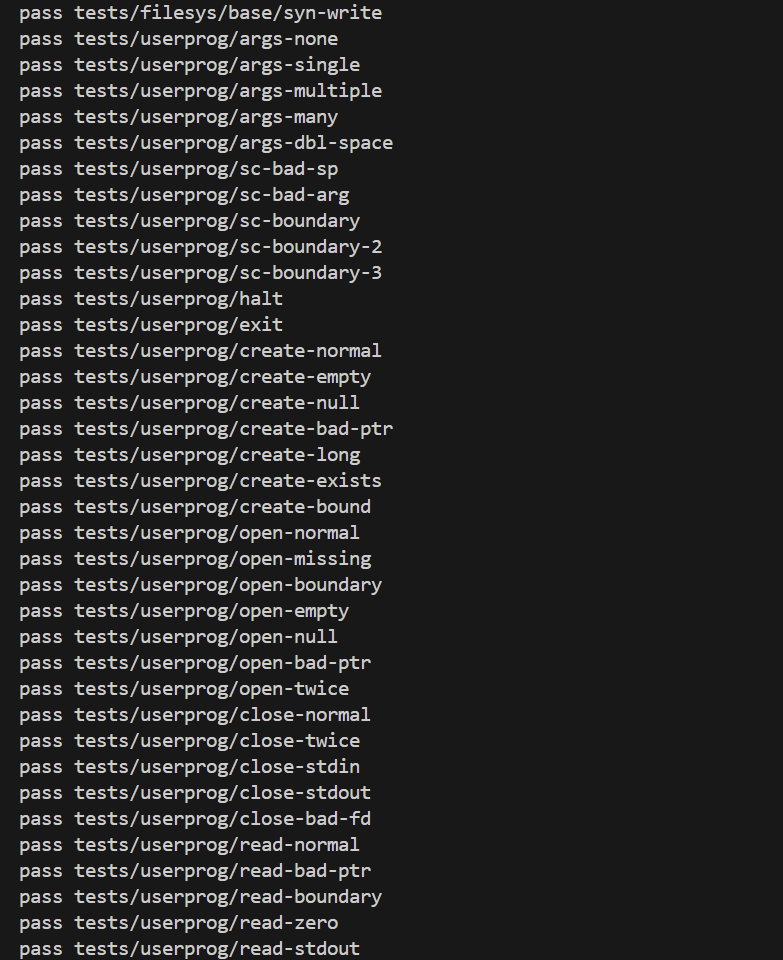
\includegraphics[width=\textwidth]{images/2.after_proj_1.jpg}
			\caption{after\_proj - 1}
		\end{minipage}
		\hfill
		\begin{minipage}[b]{0.45\textwidth}
			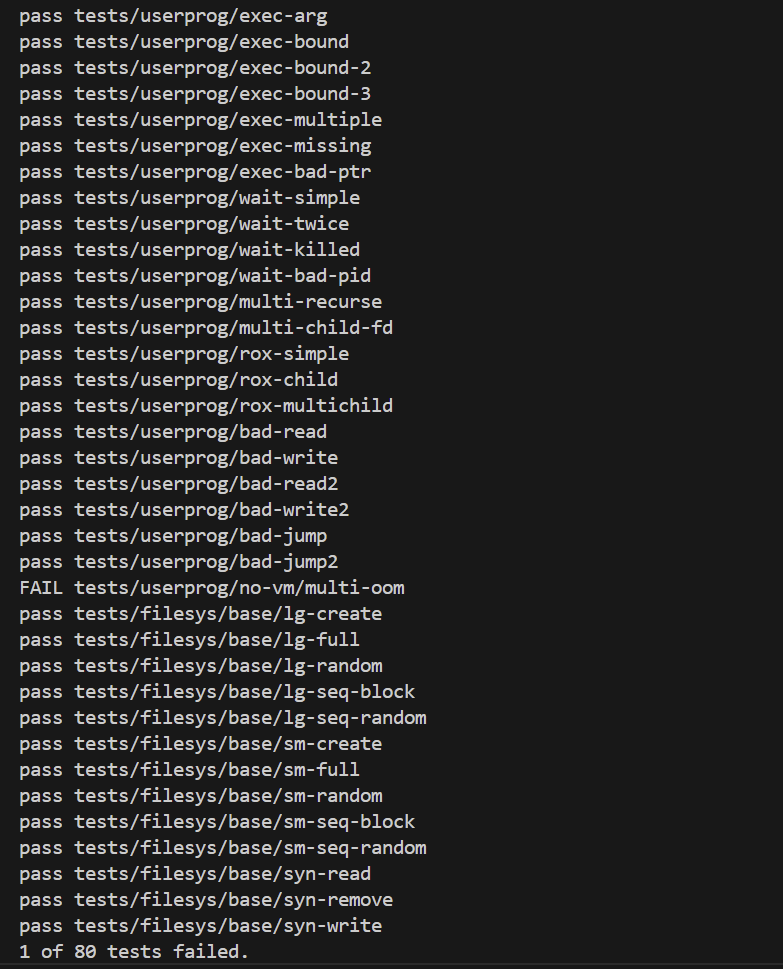
\includegraphics[width=\textwidth]{images/2.after_proj_2.jpg}
			\caption{\texttt{after\_proj - 2}}
		\end{minipage}
	\end{figure}
	
	实验的具体过程分析参考上文的第二章节部分。
	
	通过diff -urNa ~/original-pintos/ ~/pintos/ > project2.527.GuYiwei.patch 之后,得到补丁文件,部分内容如下图所示:
	
	\begin{figure}[h]
		\centering
		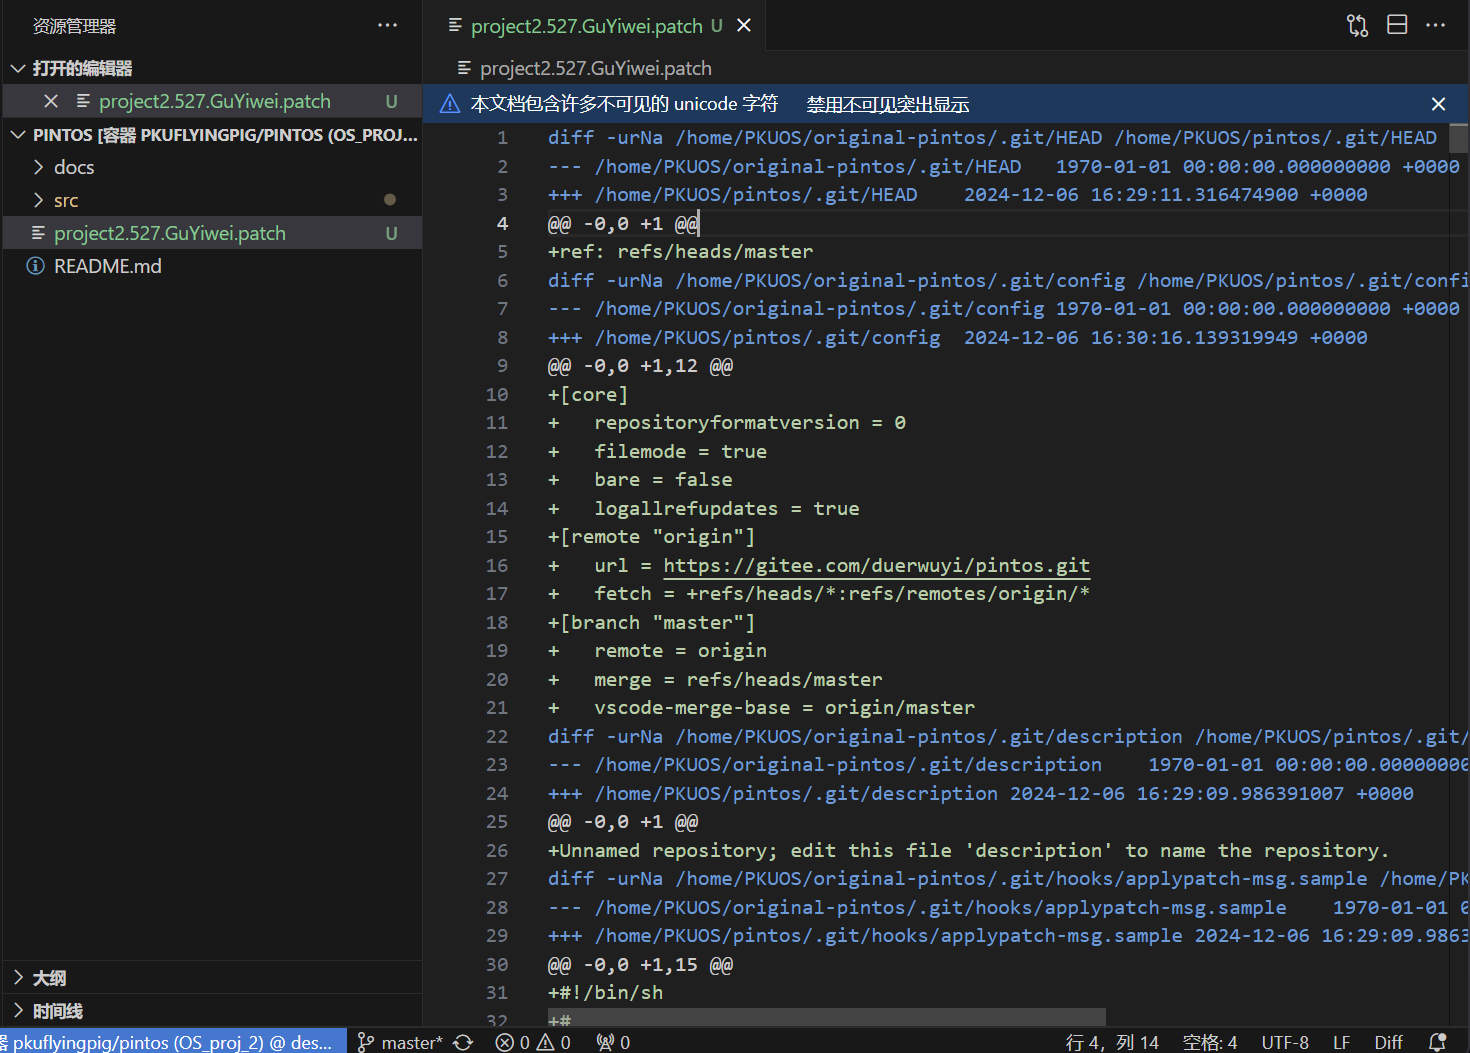
\includegraphics[width=10cm]{./images/3.patch文件.jpg}
		\caption{patch文件}
		\label{fig:graph3}
	\end{figure}
	
	\section{实验结果总结}
	
	本次实验里,我完成了参数传递和系统调用共13个函数的实现,这个实验让我对操作系统的进程管理、内存管理和文件系统管理都有了更深入的了解。
	
	\section{附录(源代码)}
	
	见上传的附件中的src压缩包内的内容。
	
	也可以访问:https://github.com/SoftGhostGU/In\_class\_related/tree/main/操作系统\_project/Proj2
\end{document}